% Options for packages loaded elsewhere
\PassOptionsToPackage{unicode}{hyperref}
\PassOptionsToPackage{hyphens}{url}
%
\documentclass[
  ignorenonframetext,
]{beamer}
\usepackage{pgfpages}
\setbeamertemplate{caption}[numbered]
\setbeamertemplate{caption label separator}{: }
\setbeamercolor{caption name}{fg=normal text.fg}
\beamertemplatenavigationsymbolsempty
% Prevent slide breaks in the middle of a paragraph
\widowpenalties 1 10000
\raggedbottom
\setbeamertemplate{part page}{
  \centering
  \begin{beamercolorbox}[sep=16pt,center]{part title}
    \usebeamerfont{part title}\insertpart\par
  \end{beamercolorbox}
}
\setbeamertemplate{section page}{
  \centering
  \begin{beamercolorbox}[sep=12pt,center]{part title}
    \usebeamerfont{section title}\insertsection\par
  \end{beamercolorbox}
}
\setbeamertemplate{subsection page}{
  \centering
  \begin{beamercolorbox}[sep=8pt,center]{part title}
    \usebeamerfont{subsection title}\insertsubsection\par
  \end{beamercolorbox}
}
\AtBeginPart{
  \frame{\partpage}
}
\AtBeginSection{
  \ifbibliography
  \else
    \frame{\sectionpage}
  \fi
}
\AtBeginSubsection{
  \frame{\subsectionpage}
}
\usepackage{amsmath,amssymb}
\usepackage{iftex}
\ifPDFTeX
  \usepackage[T1]{fontenc}
  \usepackage[utf8]{inputenc}
  \usepackage{textcomp} % provide euro and other symbols
\else % if luatex or xetex
  \usepackage{unicode-math} % this also loads fontspec
  \defaultfontfeatures{Scale=MatchLowercase}
  \defaultfontfeatures[\rmfamily]{Ligatures=TeX,Scale=1}
\fi
\usepackage{lmodern}
\usetheme[]{metropolis}
\usecolortheme{seahorse}
\ifPDFTeX\else
  % xetex/luatex font selection
\fi
% Use upquote if available, for straight quotes in verbatim environments
\IfFileExists{upquote.sty}{\usepackage{upquote}}{}
\IfFileExists{microtype.sty}{% use microtype if available
  \usepackage[]{microtype}
  \UseMicrotypeSet[protrusion]{basicmath} % disable protrusion for tt fonts
}{}
\makeatletter
\@ifundefined{KOMAClassName}{% if non-KOMA class
  \IfFileExists{parskip.sty}{%
    \usepackage{parskip}
  }{% else
    \setlength{\parindent}{0pt}
    \setlength{\parskip}{6pt plus 2pt minus 1pt}}
}{% if KOMA class
  \KOMAoptions{parskip=half}}
\makeatother
\usepackage{xcolor}
\newif\ifbibliography
\setlength{\emergencystretch}{3em} % prevent overfull lines
\providecommand{\tightlist}{%
  \setlength{\itemsep}{0pt}\setlength{\parskip}{0pt}}
\setcounter{secnumdepth}{-\maxdimen} % remove section numbering
\usepackage{xcolor}
\definecolor{myorange}{RGB}{255, 94, 77}
\setbeamertemplate{footline}{}
\usepackage{bookmark}
\IfFileExists{xurl.sty}{\usepackage{xurl}}{} % add URL line breaks if available
\urlstyle{same}
\hypersetup{
  pdftitle={Graphical Integrity},
  pdfauthor={(\textbackslash text\{Professor Dave\})\^{}2},
  hidelinks,
  pdfcreator={LaTeX via pandoc}}

\title{Graphical Integrity}
\author{\((\text{Professor Dave})^2\)}
\date{}
\institute{The University of Austin}

\begin{document}
\frame{\titlepage}

\begin{frame}{Introduction}
\phantomsection\label{introduction}
Most of the material comes from Chapter 2 of \emph{``The Visual Display
of Quantitative Information''} by Edward R. Tufte (2nd Edition, Graphics
Press, 2007).

\begin{columns}
\column{0.5\textwidth}
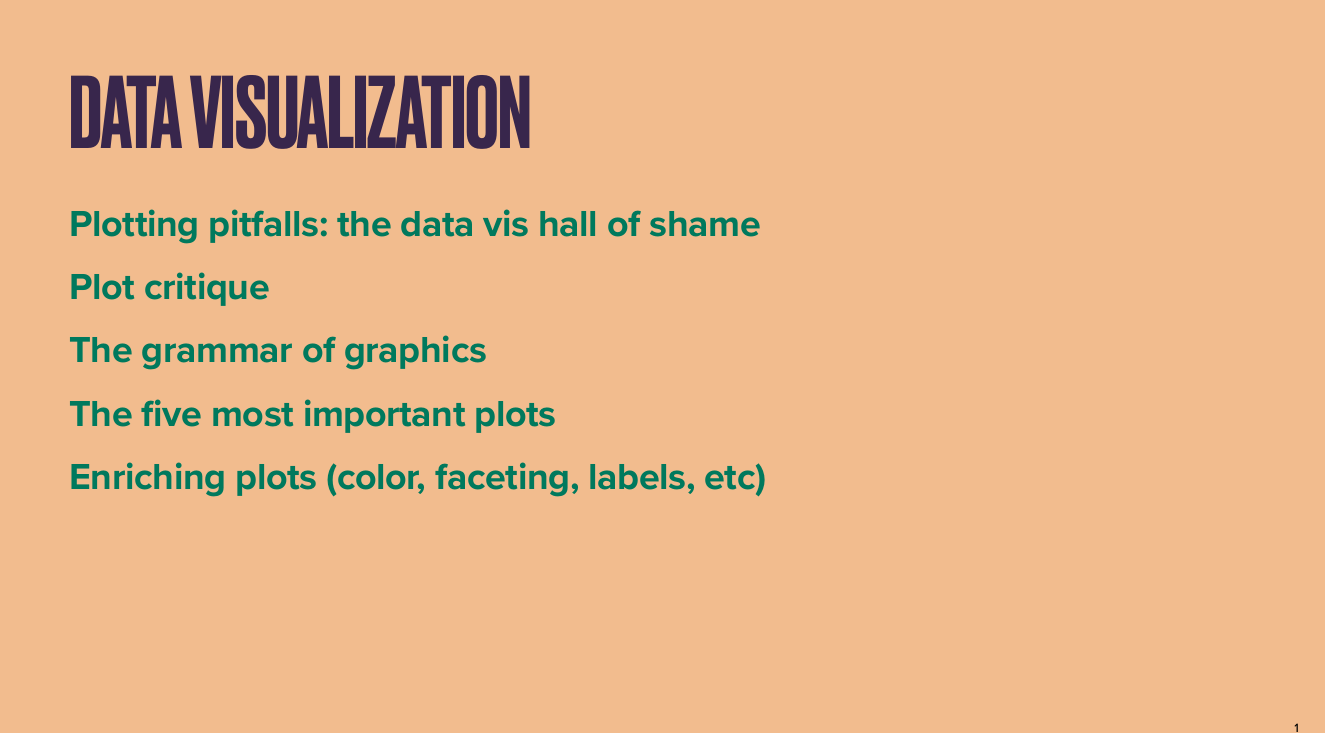
\includegraphics[width=\textwidth]{{integrity_figs/fig_1.png}}
\column{0.5\textwidth}
Integrity translates into telling the truth with a graph. Most graph users in the 20th century focused on catching lies rather than analyzing data.
\end{columns}
\end{frame}

\begin{frame}{Lying with Graphs}
\phantomsection\label{lying-with-graphs}
\begin{columns}
\column{0.5\textwidth}
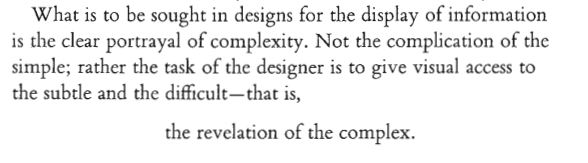
\includegraphics[width=\textwidth]{{integrity_figs/fig_2.png}}
\column{0.5\textwidth}
Let’s start with some examples of how graphs can lie.
\end{columns}
\end{frame}

\begin{frame}{Negative Income Example}
\phantomsection\label{negative-income-example}
\begin{columns}
\column{0.5\textwidth}
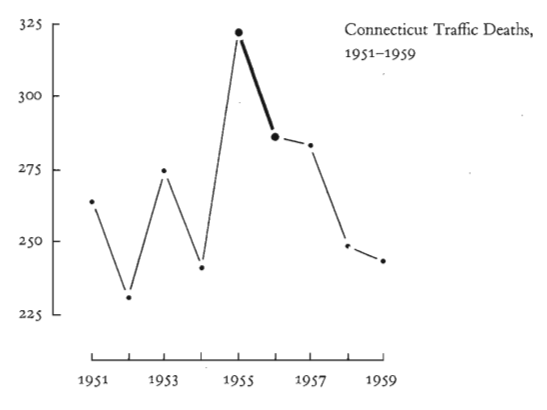
\includegraphics[width=\textwidth]{{integrity_figs/fig_3.png}}
\column{0.5\textwidth}
Negative income: Bars begin at a value of ~negative \$4.2M.
\end{columns}
\end{frame}

\begin{frame}{Time Period Misrepresentation}
\phantomsection\label{time-period-misrepresentation}
\begin{columns}
\column{0.5\textwidth}
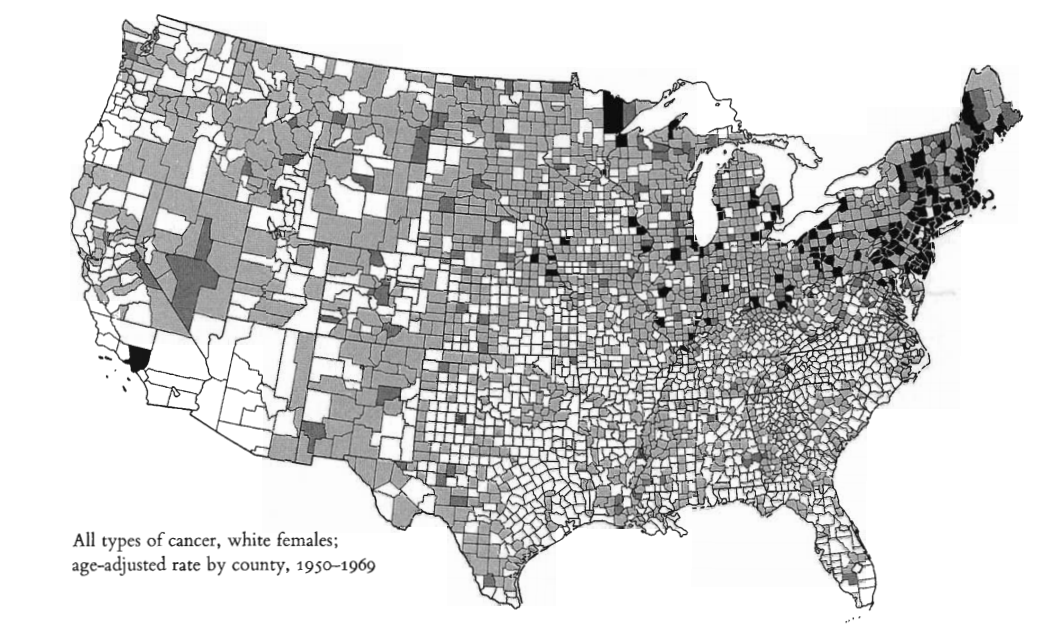
\includegraphics[width=\textwidth]{{integrity_figs/fig_4.png}}
\column{0.5\textwidth}
Periods correspond to 1976, 1977, and six months of 1978! The lie is repeated four times to conclude a decline in commission payments.
\end{columns}
\end{frame}

\begin{frame}{Disorganized Graph}
\phantomsection\label{disorganized-graph}
\begin{columns}
\column{0.5\textwidth}
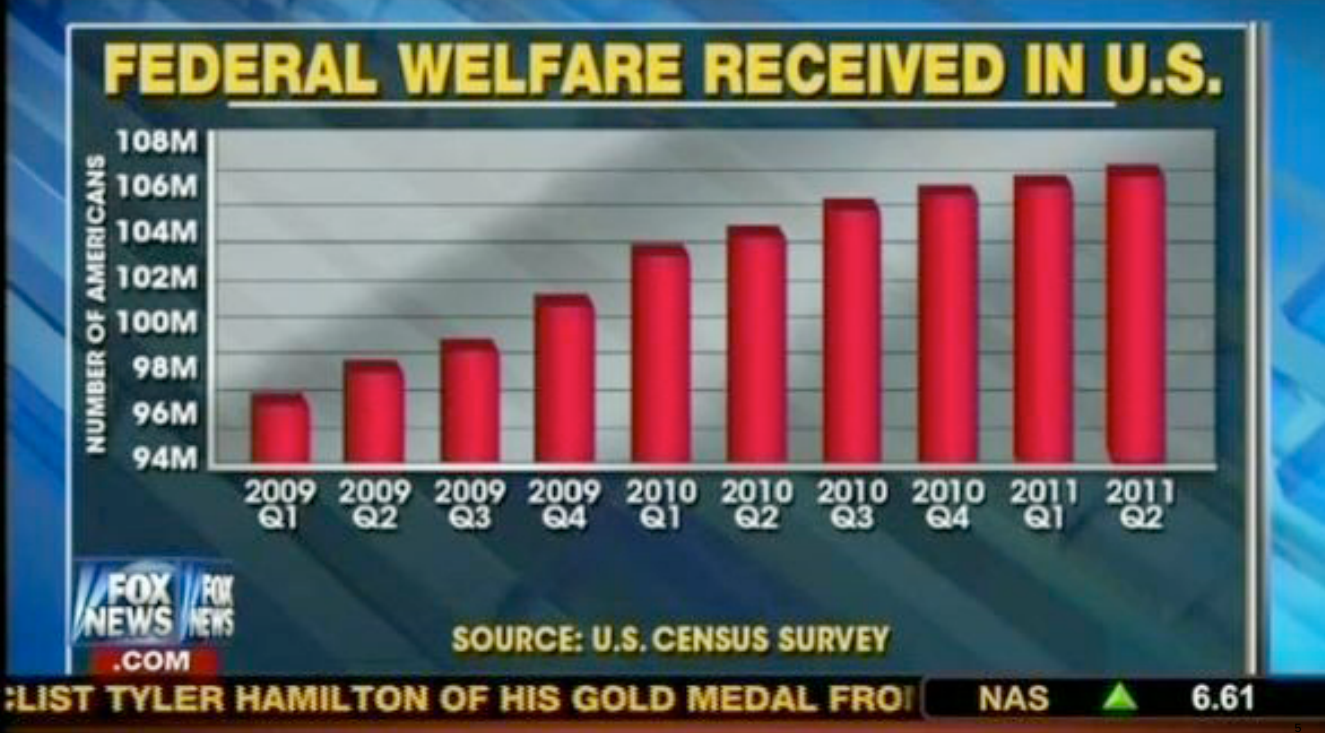
\includegraphics[width=\textwidth]{{integrity_figs/fig_5.png}}
\column{0.5\textwidth}
Notice the disorganized nature of this graph (order is ignored). Example: Pennsylvania State Hospitals.
\end{columns}
\end{frame}

\begin{frame}{Human Perception}
\phantomsection\label{human-perception}
\begin{columns}
\column{0.5\textwidth}
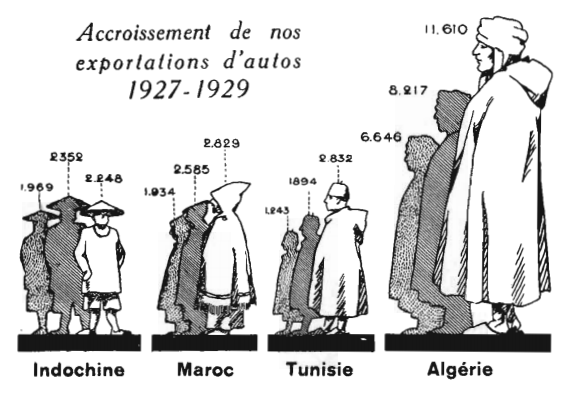
\includegraphics[width=\textwidth]{{integrity_figs/fig_6.png}}
\column{0.5\textwidth}
Humans perceive images differently according to context. They perceive area growth more slowly than actual growth.
\end{columns}
\end{frame}

\begin{frame}{The Lie Factor (LF)}
\phantomsection\label{the-lie-factor-lf}
\begin{columns}
\column{0.5\textwidth}
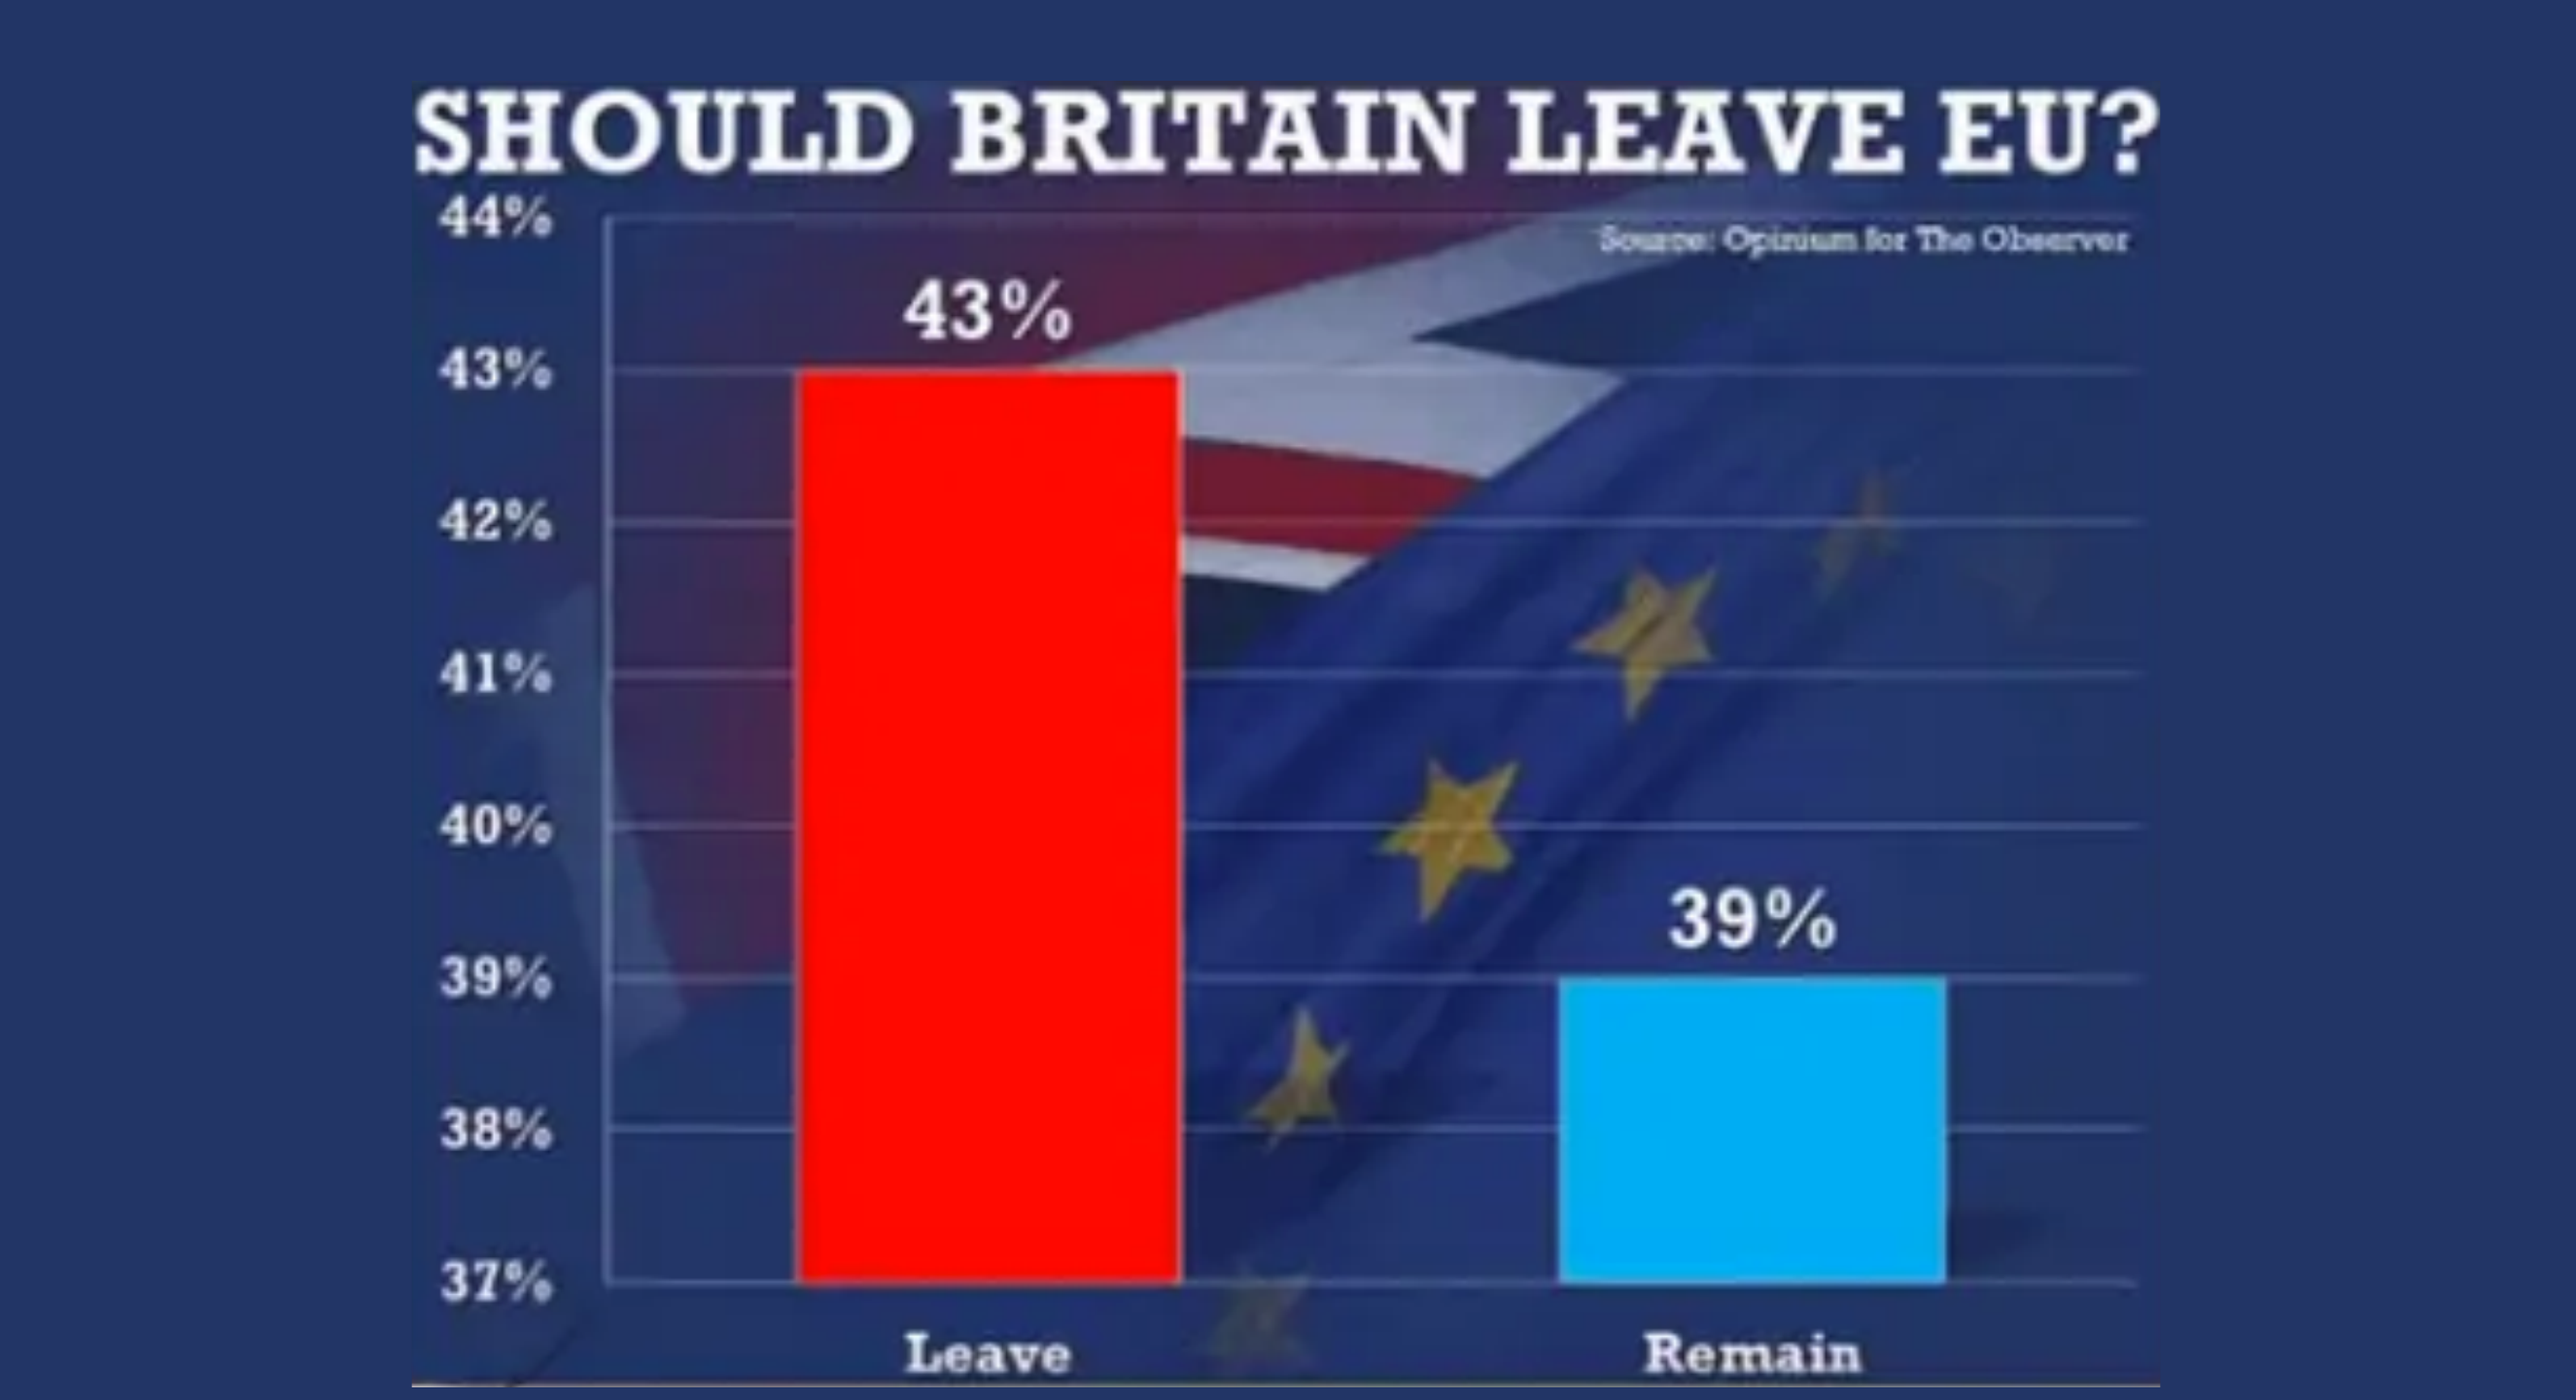
\includegraphics[width=\textwidth]{{integrity_figs/fig_7.png}}
\column{0.5\textwidth}
The Lie Factor (LF) aims for LF = 1. If LF > 1.05 or LF < 0.95, the graph is distorted. Using log(LF) helps identify overstating or understating errors.
\end{columns}
\end{frame}

\begin{frame}{Graphical Distortion}
\phantomsection\label{graphical-distortion}
\begin{columns}
\column{0.5\textwidth}
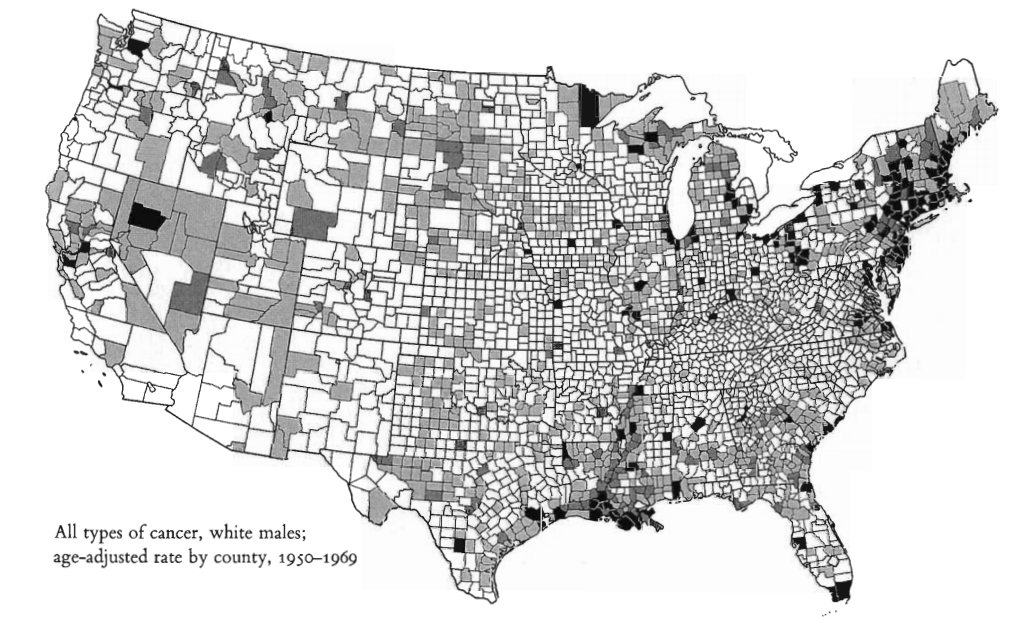
\includegraphics[width=\textwidth]{{integrity_figs/fig_8.png}}
\column{0.5\textwidth}
Example of graph distortion: Time moves in reverse order along the road to exaggerate the effect.
\end{columns}
\end{frame}

\begin{frame}{Simple Graphs}
\phantomsection\label{simple-graphs}
\begin{columns}
\column{0.5\textwidth}
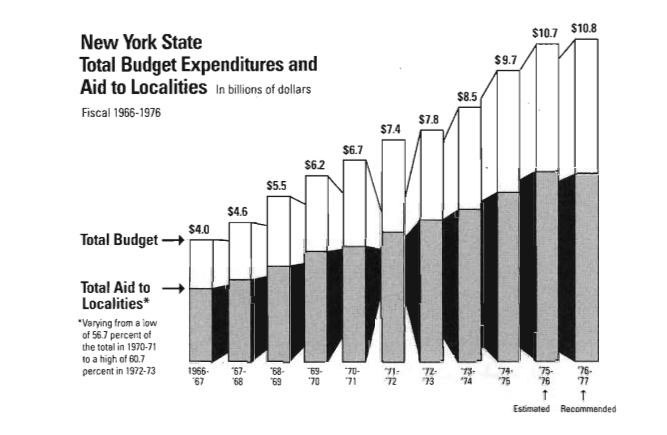
\includegraphics[width=\textwidth]{{integrity_figs/fig_9.png}}
\column{0.5\textwidth}
Choose simple graphs that are clear, precise, and don't lie. Example: Baseline for comparison adds context.
\end{columns}
\end{frame}

\begin{frame}{The remaining slides will follow the same structure using
the extracted figures.}
\phantomsection\label{the-remaining-slides-will-follow-the-same-structure-using-the-extracted-figures.}
\end{frame}

\begin{frame}{(This template includes 9 slides, but the final output
will contain the full sequence up to slide 26 with all figures.)}
\phantomsection\label{this-template-includes-9-slides-but-the-final-output-will-contain-the-full-sequence-up-to-slide-26-with-all-figures.}
\end{frame}

\end{document}
